% !TEX root = ../thesis.tex

% Tässä osassa esitetään tulokset ja vastataan tutkielman alussa
% esitettyihin tutkimuskysymyksiin. Tieteellisen kirjoitelman
% arvo mitataan tässä osassa esitettyjen tulosten perusteella.

% You have done your work, but that’s1 not enough.
% You also need to evaluate how well your implementation works. The
% nature of the evaluation depends on your problem, your method, and your
% implementation that are all described in the thesis before this chapter. If
% you have created a program for exact-text matching, then you measure how
% long it takes for your implementation to search for different patterns, and
% compare it against the implementation that was used before. If you have
% designed a process for managing software projects, you perhaps interview
% people working with a waterfall-style management process, have them adapt
% your management process, and interview them again after they have worked
% with your process for some time. See what’s changed.
% The important thing is that you can evaluate your success somehow.
% Remember that you do not have to succeed in making something spectacular;
% a total implementation failure may still give grounds for a very good master’s
% thesis—if you can analyze what went wrong and what should have been done.

\documentclass[thesis.tex]{subfiles}

\begin{document}

\chapter{Experiment}
\label{chapter:experiment}

The purpose of the experiment was to investigate the feasibility and performance (precision) of photoluminescence-based product authentication using the fingerprint method described in the previous chapter. To gain better understanding of the overall performance of the pipeline an additional set of results was computed by substituting the fingerprint analysis and matching steps with a more computationally intensive histogram-based approach. This approach is discussed in more detail in Chapter \ref{chapter:results}. The following Chapter \ref{chapter:setup} introduces the luminophores, the hardware and the various capture, analysis and matching parameters used in the experiment. The results for both the fingerprint and the histogram-based methods are summarized and compared in Chapter \ref{chapter:results}. Finally, some artefacts introduced by the capture pipeline are presented.

\section{Setup}
\label{chapter:setup}

The luminophores used for the experiment were LumiNova\textregistered\ red (O), green (G) and blue (DB) pigments. Each of the pigments was mixed with a \emph{transparent carrier} to form a stock solution. The stock solutions were pipeted in increments of $50\mu l$ onto white blank cartons to form eight unique taggants. Two samples ($a$ and a replicate sample $b$) were taken from each solution, so a total of 16 different taggants were prepared for the experiment. The taggants and the amount of phosphor and transparent carrier used to create them are listed in Appendix \ref{appendix:taggants}. For information about the chemical properties of the LumiNova\textregistered\ pigments the reader is referred to \cite{luminova}.

The taggants were captured using Samsung S4 (version 4.4.2) and Lumia 1020 (version WP8.1) smartphones. The MFD of the S4 and the 1020 was determined empirically to be around 100mm and 150mm, respectively. The height of the camera module was adjusted accordingly to ensure that no image blur would be introduced. As depicted in Figure \ref{figure:camera_module} the light source was positioned perpendicular to the taggant as per the common conventions in fluorescense spectoscopy \cite{spectroscopy-principles}. Yongnuo YN565EX\footnote{Yongnuo YN565EX User Manual: \url{http://www.yongnuo.com.cn/usermanual/pdf/USER_MANUAL_YN565EX_EN.pdf}} external camera flash was used as the light source as it provided a convenient way to produce a high quality, full-spectrum white light for the photoexcitation. The power and zoom level of the flash were set to 1/32 and 24mm, respectively. The zoom level of the flash was set to the widest supported level assuming that the taggant would be more suspectible to uneven exposure on higher levels of zoom due to a more concentrated burst of light. The power level of 1/32 was selected by observing at which level the captured frames would no longer be subject to overexposure.

In total, nine different capture presets were defined: six presets for the Samsung S4 (prefixed $an$) and three presets for the Lumia 1020 ($wp$). The capture presets and the corresponding parameter values are listed in Appendix \ref{appendix:capture-presets}. The parameter values are discussed more thoroughly in Chapter \ref{chapter:discussion}. All of the 16 taggants were captured with each of the presets resulting in a corpus of 144 fingerprints. The fingerprints were labeled based on the capture preset and the taggant in the following format: \emph{\{preset\}/\{taggant\}\{sample\}} (e.g. \emph{wp200/Sa}). A subset of the taggants captured with the Samsung S4 and Lumia 1020 are presented in Figure \ref{figure:taggants} for preview.

\begin{figure}[h]
\label{figure:taggants}
\centering 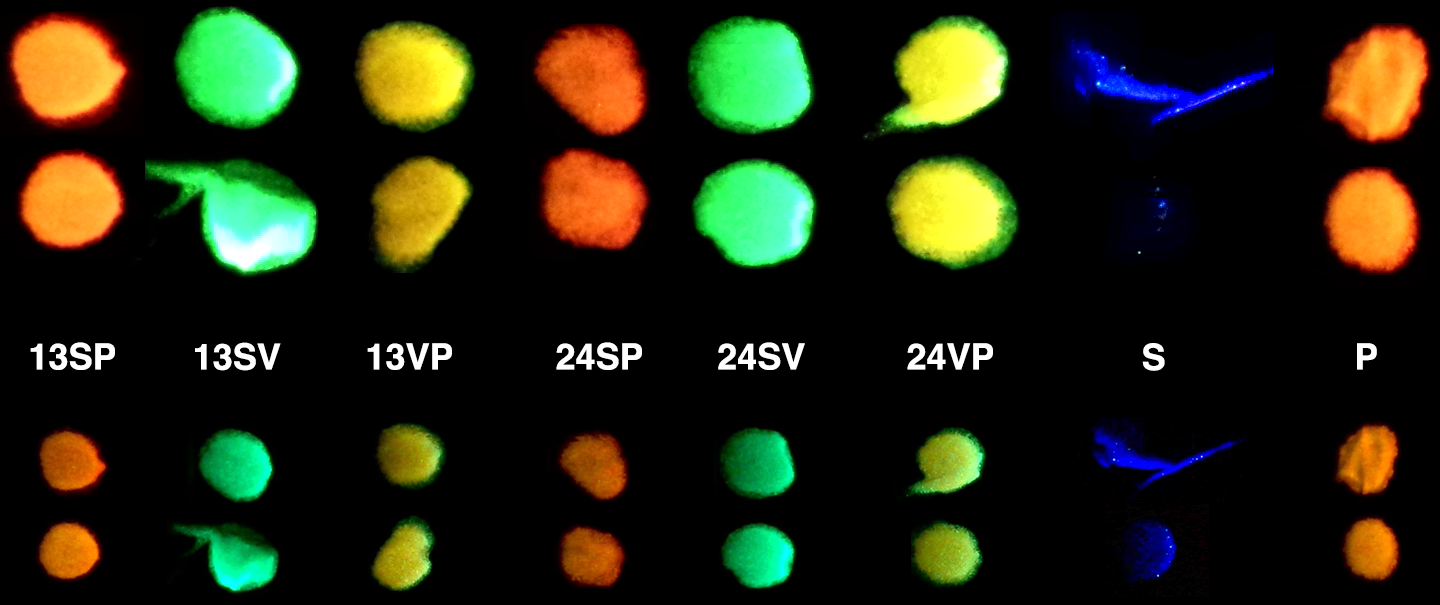
\includegraphics[width=\textwidth,height=\textheight,keepaspectratio=true]{images/experiment/taggants}
\caption{Captured taggant samples \emph{a} (upper) and \emph{b} (lower) for both the Samsung S4 (top two rows) and the Lumia 1020 (bottom two rows).}
\end{figure}
\clearpage

The taggants were captured in a dimly lit room to minimize interference of ambient light. After capture, each taggant was given 15 minutes to reset to ground state in order to minimize the effect of residual afterglow on subsequent captures.

\section{Results}
\label{chapter:results}

The performance of the fingerprint pipeline was evaluated by computing the similarity score of each fingerprint against the rest of the corpus. The lowest score (best) was expected to be given to the fingerprint's countersample (sample \emph{a} or \emph{b}). For example, for fingerprint \emph{an200/24SPa} the closest match was expected to be \emph{an200/24SPb}. For fingerprints captured with the Samsung S4 the resolution variant and its countersample were also considered a match. That is, for \emph{an200/24SPa} valid matches would actually include three fingerprints: \emph{an200/24SPb}, \emph{an200r/24SPa} and \emph{an200r/24SPb}. For brevity, valid matches of a fingerprint are henceforth referred to as \emph{sibling fingerprints}.

The similarities were computed using the fingerprint matching algorithm presented in Chapter \ref{chapter:fingerprint-matching} and a more computationally intensive histogram-based method, results of which could be used to assess the performance of the fingerprint matching algorithm. The histogram method was implemented using the \emph{compareHist()} function of OpenCV's image processing API to compute the \emph{Hellinger distance} between two histograms. As input, the function was given the Hue-Saturation histograms of the frames of two fingerprints \emph{A} and \emph{B} frame-by-frame. The sum of the computed Hellinger distances denoted the similarity between the two fingerprints -- the lower sum, the better a match. Hellinger distance was chosen as the comparison method as it is considered a de facto approach for comparing probability distributions (e.g. histograms) \cite{hellinger}. To avoid ambiguity the fingerprint analysis and matching process and the histogram-based approach are henceforth referred to as \emph{fingerprint} and \emph{histogram methods}. The method parameter values used in the experiment are summarized in Appendix \ref{appendix:method-parameters}.

For both methods the computed similarity scores were consolidated into a $n\times n$ similarity matrix, where $n$ was equal to the number of fingerprints in the corpus (144) and each row/column represented the similarity of a fingerprint to the rest of the corpus. The resulting matrix would thus be a \emph{zero-diagonal symmetric matrix}. The similarity matrices were first used for finding fingerprint clusters. The clusters would indicate -- on a broad level -- how accurate the given method was. Ideally, the clustering would produce 48-72 clusters (one for each group of sibling fingerprints) each consisting of 1-3 sibling fingerprints. The results of the clustering are visualized in Figure \ref{figure:clusters} (each cluster includes its exemplar, too). Each bar in the graphic represents a fingerprint, where the color denotes the taggant and height the interval duration. That is, the clusters would ideally be of equal color and height, forming a group of sibling fingerprints. It should be noted that the visualization distinguishes presets only by the difference in the interval duration. Thus, for example the preset platform a given fingerprint was captured under (Android/Windows Phone) is not communicated by the visualization.

\begin{figure}[h]
\label{figure:clusters}
\centering 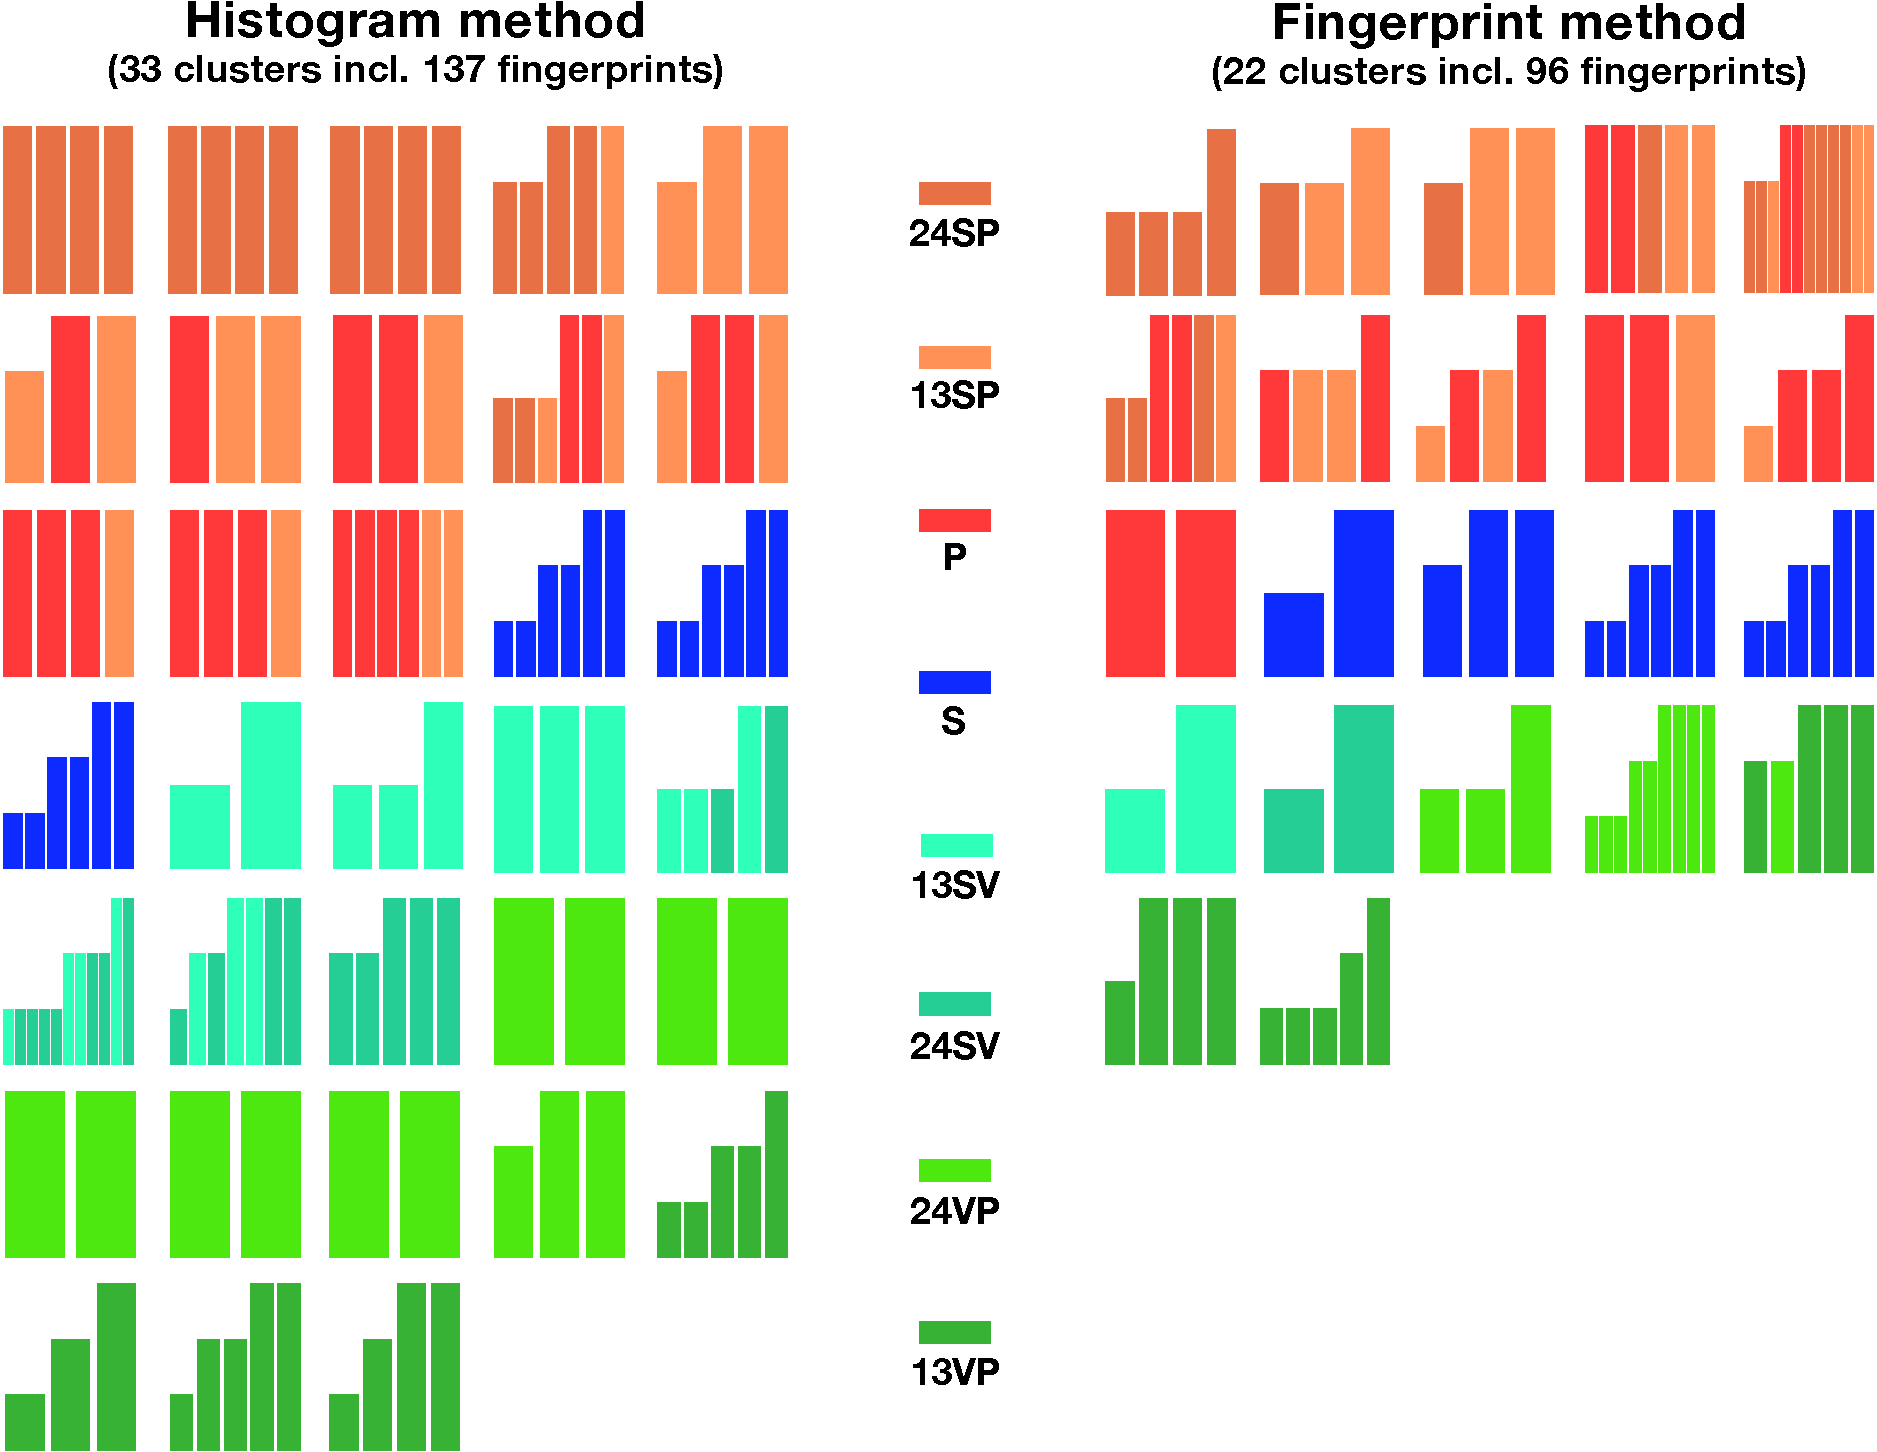
\includegraphics[page=1,width=\textwidth,height=\textheight,keepaspectratio=true]{images/experiment/clusters}
\caption{Fingerprint clusters based on the similarities computed by the histogram and fingerprint methods. Each bar represents a fingerprint, where the color denotes the taggant and height the interval duration.}
\end{figure}

The fingerprints were clustered using affinity propagation (AP) and its implementation in R\footnote{\url{http://cran.at.r-project.org/web/packages/apcluster}}. The benefit of AP clustering is that no apriori knowledge of the number of clusters to be computed is required. It is best suited for small to medium-sized datasets as it is computationally heavier than most other clustering algorithms. The similarity matrices were processed by the algorithm using the default values for all parameters except for the \emph{q} parameter (sample quantile threshold), which was set to $q=0.95$. The sample quantile threshold ($0-1$) can be used to adjust how aggressively the algorithm clusters the data -- the higher the value, the more clusters the algorithm tries to find. For further information about AP clustering and its R implementation the reader is referred to \cite{affinity_propagation}.

To gain more insight into how well the methods rank the fingerprints -- that is, match fingerprints' with their respective siblings -- a pair of \emph{boundary conditions} needs to be established. Based on the boundary conditions candidate fingerprints are either qualified or disqualified. The first boundary condition is the \emph{maximum number} of candidate fingerprints to qualify, $B_{count}$. However, $B_{count}$ alone does not suffice. For example, the top five candidates for a fingerprint might well be very far apart of each other in terms of similarity (score). Therefore, to evaluate how similar the best candidates are, they need to be further constrained by a margin, $B_{margin}$. For example, given a margin of 30\% only candidates whose similarity score is within a 30\% margin of the score of the best candidate qualify. Together the two boundary conditions, $B_{count}$ and $B_{margin}$, provide an unambiguous way to determine, which candidate fingerprints should be considered a match.

Figures \ref{figure:match_precision_fingerprint} and \ref{figure:match_precision_histogram} present the \emph{success rate} and \emph{precision} of the fingerprint and histogram methods as a function of $B_{margin}$ for different $B_{count}$. Success rate describes the ratio of the corpus fingerprints, for which the matches found included at least one sibling fingerprint. The ratio of sibling fingerprints among these matches is given by precision. For example, when out of the top six candidates ($B_{count}=6$) only those that were within a 75\% margin ($B_{margin}=0.75$) of the best match were qualified, approximately $59\%$ of the cases included at least one valid match (a sibling fingerprint), and in each case approximately $53\%$ of the matches were relevant (siblings).

The results for $B_{count}=1$ are omitted from the graphs, and instead, presented in Table \ref{table:match_precision_count1} with a few additional statistics. \emph{Matched Taggant} and \emph{Matched Preset} describe the ratio of cases where the fingerprint corresponded its matches either only by the taggant or preset. \emph{Misses} represent cases where neither the taggant nor the preset of the matches corresponded the subject fingerprint. In a few cases more than one of a fingerprint's candidates would be given the same best score resulting in situation where the number of matches could potentially be greater than $B_{count}$. The fingerprint method clearly exhibits this behaviour as the precision is less than 100\% already at $B_{count}=1$.

Let $M_n$ represent the margin, within which the top $n$ matches (or less) of a fingerprint fit. Figure \ref{figure:match_precision_margin} presents per method the mean and standard deviation of $M_4$ as a function of $B_{margin}$. For example, when the top four matches (or less) within a 50\% boundary margin ($B_{margin}=0.5$) of the best match would be qualified, $M_4$ was on average 17\% and 31\% for the fingerprint and histogram methods, respectively.

Figure \ref{figure:tags_presets} provides a summary of the total number of matches per taggant and preset for $B_{count}$ of 3, 4 and 6. The $B_{margin}$ values of 75\% (for the fingerprint method) and 30\% (for the histogram method) were selected based on when the methods reach identical precision at $B_{count}=4$ ({\raise.17ex\hbox{$\scriptstyle\sim$}}55\%). Capture artefacts encountered during the experiment are summarized in Figure \ref{figure:artefacts}.

\begin{figure}[h!]
  \centering 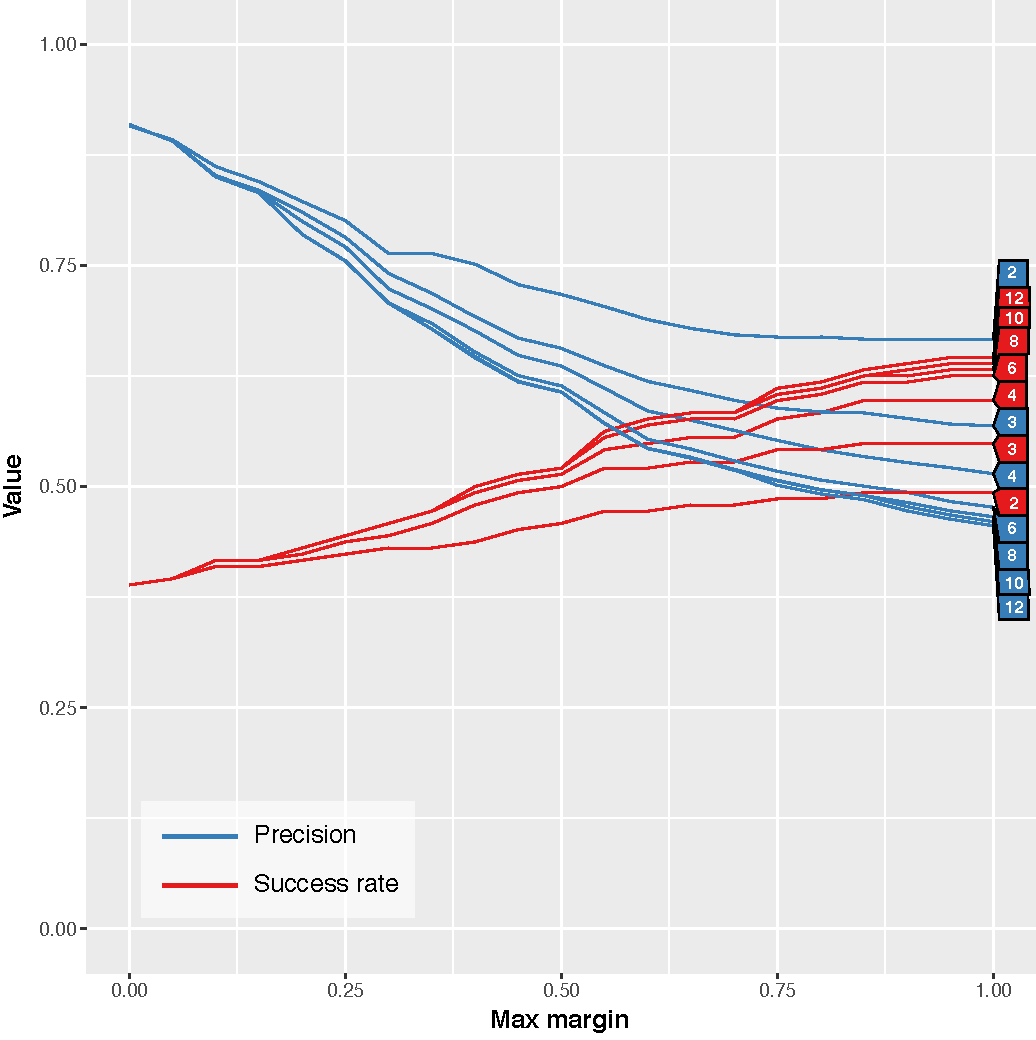
\includegraphics[page=1,width=\textwidth]{images/experiment/match_precision}
  \vspace{-9mm}
  \caption{Success rate and precision of the fingerprint method for different $B_{count}$ as a function of $B_{margin}$.}
  \label{figure:match_precision_fingerprint}
\end{figure}

\begin{figure}[h]
\centering \includegraphics[page=2,width=\textwidth,height=\textheight,keepaspectratio=true]{images/experiment/match_precision}
\vspace{-9mm}
\caption{Success rate and precision of the histogram method for different $B_{count}$ as a function of $B_{margin}$.}
\label{figure:match_precision_histogram}
\end{figure}

\clearpage

\begin{table}[b]
  \caption{Statistics per method when only the best fingerprint candidate is qualified ($B_{count} = 1$). Histogram method outperforms the fingerprint method in all aspects.}
  \label{table:match_precision_count1}

  \begin{center}
  \begin{tabular}{| c | c | c |}
    \hline
    \textbf{Method} & Fingerprint & Histogram \\
    \hline
    \textbf{Success Rate} & 37,50\% & 44,44\% \\
    \hline
    \textbf{Precision} & 93,52\% & 100\% \\
    \hline
    \textbf{Matched Taggant} & 75,69\% & 88,89\% \\
    \hline
    \textbf{Matched Preset} & 55,56\% & 70,39\% \\
    \hline
    \textbf{Misses} & 12,50\% & 6,25\% \\
    \hline
  \end{tabular}
  \end{center}
\end{table}

\begin{figure}[t]
\centering \includegraphics[page=3,width=\textwidth,height=\textheight,keepaspectratio=true]{images/experiment/match_precision}
\caption{Mean and standard deviation of the margin, within which a subject fingerprint's matches fit when $B_{count}=4$.}
\label{figure:match_precision_margin}
\end{figure}

\begin{figure}[t]
\centering \includegraphics[page=7,width=0.99\textwidth,height=\textheight,keepaspectratio=true]{images/experiment/tags_configs}
\vspace{-3mm}
\caption{Total number of matches per preset and taggant for different $B_{count}$. The results of the fingerprint (left) and histogram (right) methods are computed using a different $B_{margin}$: 75\% and 30\%, respectively.}
\label{figure:tags_presets}
\end{figure}

\begin{figure}[b]
\centering \includegraphics[page=2,width=0.85\textwidth,height=\textheight,keepaspectratio=true]{images/experiment/artefacts}
\vspace{-3mm}
\caption{The Samsung S4 focus light, non-uniform luminophore concentration and the interference of the light source introduced capture artefacts.}
\label{figure:artefacts}
\end{figure}


\end{document}